\chapter{Himmelsmechanik}
\section{Kinematik}
\subsection*{vor Newton}
\begin{description}
    \item[Aufgabe] genaue Beschreibung der scheinbaren Bewengung
        \begin{itemize}
            \item \emph{nicht} die Erklärung/das Verständnis des zugrunde
                  liegenden Sachverhaltes (Gesetztes)
        \end{itemize}
    \item[speziell] scheinbare Planetenbahnen $\rightarrow$ Mars
        \begin{center}
            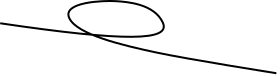
\includegraphics[width=.3\textwidth]{img/ptolemaeus_mars.pdf}
        \end{center}
    \item[Modelle]
        \begin{itemize}
            \item \textsc{Ptolemäus:}
                \begin{itemize}
                    \item Geozentrisch (Erde im Zentrum)
                    \item Planeten auf Epizykelbahnen
                \end{itemize}
            \item \textsc{Kopernikus:}
                \begin{itemize}
                    \item Heliozentrisch (Sonne im Zentrum)
                    \item \emph{Kreisbahnen}
                \end{itemize}
        \end{itemize}
    \item[Enscheidung] z. B. Planetenphasen der inneren Planeten\\
        $\Rightarrow$ Kopernisches Weltbild
\end{description}
\begin{itemize}
    \item \textsc{Kepler:} Messung d. Marsbahnen (T. \textsc{Brahe})\\
          $\Rightarrow$ \textsc{Kepler}'sche Gesetze (empirisch)
          \begin{enumerate}
              \item Ellipsen, Sonne in einem Brennpunkt
              \item Flächensatz $\Leftrightarrow$ Drehimpulserhaltung \\
                    Radiusvektoren überstreichen in gleicher Zeit gleiche Flächen,\\
                    d. h. Flächengeschwindigkeit = $\mathbf{const}$
              \item Umlaufzeiten/Abstände ($a$: Halbachse, $T$: Umlaufzeit)
                      \[ \frac{a^3}{T^2} \sim \mathbf{const} \]
          \end{enumerate}
\end{itemize}

\section{\textsc{Newton}'sche Mechanik}
\subsection{\textsc{Newton}'sche Axiome}
\begin{enumerate}[(i)]
    \item Trägheitsgesetz (Masse konstant, vergl. spezielle Relativitätstheorie):
        \begin{equation}
            \vec p = m \vec v = m \dot{\vec{r}} = m \frac{d}{dt} \vec r
            \label{eq:newton1}
        \end{equation}
    \item Impulsänderung durch Krafteinwirkung:
        \begin{equation}
            \frac{d}{dt} \vec p = \dot{\vec p} = \vec F = m \ddot{\vec r} = m \frac{d^2}{dt^2} \vec r = m \vec a
            \label{eq:newton2}
        \end{equation}
    \item Actio = Reactio:
        \begin{equation}
            \vec F_{ik} = -\vec F_{ki}
            \label{eq:newton3}
        \end{equation}
\end{enumerate}

\subsection{\textsc{Newton}'sche Gravitationsgesetze}
\noindent Formulierung für 2 Punktvektoren $m_1, m_2$
\paragraph{Skizze}
\begin{center}
        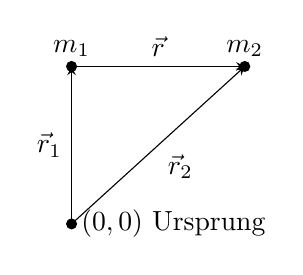
\begin{tikzpicture}[vector/.style={->}, >=stealth, auto]
            \coordinate [label=right:{$(0,0)$ Ursprung}] (O) at (0,0);
            \coordinate [label=above:$m_1$] (m1) at (0,2);
            \coordinate [label=above:$m_2$] (m2) at (2.2,2);

            \foreach \point in {O,m1,m2}
                \fill (\point) circle (2pt);
            \draw[vector] (O) -- (m1) node[align=center, midway] {$\vec r_1$};
            \draw[vector] (O) -- (m2) node[swap, align=center, midway] {$\vec r_2$};
            \draw[vector] (m1) -- (m2) node[align=center, midway] {$\vec r$};
        \end{tikzpicture}
        \begin{minipage}[b]{0.3\textwidth}
            \begin{align*}
                \vec r &= \vec r_1 - \vec r_2 \\
                |\vec r| &= r\\
                m &= m_1 + m_2
            \end{align*}
        \end{minipage}
\end{center}

\begin{equation}
    \boxed{\vec F = -\frac{G m_1 m_2 \vec r}{r^3}}
\end{equation}

\noindent $G$: \textsc{Newton}'sche Gravitationskonstante (vgl. \textsc{Einstein}'sche Gravitationskonstante $\kappa$)\\[0.5em]
\noindent Zweikörperproblem: Erhaltungsgrößen; Mit \autoref{eq:newton2} und \autoref{eq:newton3}:
\begin{equation}
    \boxed{m_1 \ddot \vec{r}_1 = \frac{G m_1 m_2 \vec r}{r^3},\qquad m_2 \ddot \vec{r}_2 = -\frac{G m_1 m_2 \vec r}{r^3}}
    \label{eq:newton_two_body}
\end{equation}

\begin{description}
    \item[Addition \autoref{eq:newton_two_body}]
        \begin{align*}
            m_1\vec{r}_1 + m_2\vec{r}_2 &= \frac{d^2}{dt^2} (m_1 \vec{r}_1 + m_2 \vec{r}_2) \\
                                      0 &= \frac{d^2}{dt^2} (m_1 \vec{r}_1 + m_2 \vec{r}_2)
        \end{align*}
        Differentialgleichung 2. Ordnung in der Zeit: $\int \cdots dt$
        \[ \Rightarrow \frac{d}{dt} (m_1 \vec{r}_1 + m_2 \vec{r}_2) = \vec{C}_{1+2} = \vec{p}_1 + \vec{p}_2 = \vec{p}_{\text{ges}} \]
        3 Konstanten $\rightarrow$ Impulserhaltung
        \[ \Rightarrow (m_1 \vec{r}_1 + m_2 \vec{r}_2) = \vec{C}_1 + \vec{C}_2 \]
        3 Konstanten $\rightarrow$ Schwerpunktsatz
    \item[Subtraktion \autoref{eq:newton_two_body}]
        \begin{align*}
            -\frac{G m_1 m_2 \vec r}{i m_2 r^3} - \frac{G m_1 m_2 \vec r}{m_1 r^3} &= \frac{\cancel{m_2} \ddot \vec{r}_2}{\cancel{m_2}} - \frac{\cancel{m_1} \ddot \vec{r}_1}{\cancel{m_1}} \\
            \ddot \vec{r} = - \frac{G \vec r}{r^3} m && \text{d.h. $\ddot \vec{r} \| \vec r$ (Zentralkraft)} \tag{$| \vec r \times$}\\
            \vec r \times \ddot \vec{r} = - \frac{Gm}{r^3} \underbrace{\vec r \times \vec r}_{= \vec 0} \\
            \frac{d}{dt} \left(\vec r \times \dot{\vec{r}}\right) = \vec 0
        \end{align*}
        Differentialgleichung 1. Ordnung in der Zeit\\[1em]
        \color{OliveGreen}
        \textbf{Nebenrechnung:}
        \[ \frac{d}{dt} (\vec r \times \dot{\vec{r}}) = \underbrace{\dot{\vec{r}} \times \dot{\vec{r}}}_{= \vec 0} + \vec r \times \ddot \vec{r} \tag{Produktregel} \]
        \color{black}
        \textbf{Lösung:} $\int \cdots dt$
        \begin{align*}
            \vec r \times \dot{\vec{r}}             &= \vec{C}_3 \\
            \vec r \times \frac{m}{m} \dot{\vec{r}} &= \frac{1}{m} (\vec r \times \underbrace{m \vec v}_{\vec p})\\
                                                    &= \frac{1}{m} \underbrace{(\vec r \times \vec p)}_{\vec L} \tag{$\vec L$: Drehimpuls}
        \end{align*}
        $\Leftrightarrow$ Drehimpulserhaltung\\
        $\Leftrightarrow \dot{\vec{L}} = 0$\\
        $\Leftrightarrow \dot{\vec{L}} = \textbf{const}$\\
        Aus der Addition von \autoref{eq:newton_two_body} mit $\vec{r}_2$ bzw. $\vec{r}_1$ folgt:
        \begin{align*}
            m_1 \langle\dot{\vec{r}}_1, \ddot{\vec{r}}_1\rangle + m_2 \langle\dot{\vec{r}}_2, \ddot{\vec{r}}_2\rangle 
                &= \frac{Gm_1m_2}{r^3} \left(\langle\vec{r}, \vec{r}_1\rangle - \langle\vec{r}, \vec{r}_2\rangle\right)\\
                &= \frac{Gm_1m_2}{r^3} (\underbrace{\langle\vec{r}_2 - \vec{r}_1, \vec{r}_1\rangle - \langle\vec{r}_2 - \vec{r}_1, \vec{r}_2\rangle}_{?})\\
        \end{align*}
        \color{OliveGreen}
        \textbf{Nebenrechnung:} $i \in {1,2}$
        \[\frac{d}{dt}\dot{\vec{r}}_i^2 = \langle2\dot{\vec{r}}_i, \ddot{\vec{r}}_i\rangle \tag{Kettenregel}\]
        \color{black}
        \begin{align*}
            \frac{d}{dt}(\vec{r}_2 - \vec{r}_1) &= \langle2(\vec{r}_2 - \vec{r}_1), \dot{\vec{r}}_2 - \vec{r}_1\rangle\\ 
                                                &= -2 \left(\langle(\vec{r}_2 - \vec{r}_1), \dot{\vec{r}}_1\rangle - \langle(\vec{r}_2 - \vec{r}_1), \vec{r}_2\rangle\right)\\
                                                &= \frac{d}{dt} r^2
        \end{align*}
        Damit gilt:
        \begin{align*}
            \frac{d}{dt} \sum\limits_{i = 1}^{2} \frac{m_i}{2} \dot r^2 &= -\frac{Gm_1m_2}{2r^3} \frac{d}{dt} r^2\\
                                                                        &= -\frac{Gm_1m_2}{2r^1} \underbrace{\frac{1}{r} \frac{d}{dt} r^2}_{?} \tag{skalare Gleichung}
        \end{align*}
        \color{OliveGreen}
        \textbf{Nebenrechnung:}
        \begin{align}
            \frac{1}{r} \frac{d}{dt} r^2            &= \frac{1}{\cancel{r}} 2 \cancel{r} \dot{r} = 2 \dot{r} \label{eq:newton_nr_1}\\
            \frac{d}{dt} \left(\frac{1}{r}\right)   &= \frac{1}{r^2} 2 \dot{r} \Leftrightarrow \dot{r} = -r^2 \frac{d}{dt} \left(\frac{1}{r}\right) \label{eq:newton_nr_2}\\
            \text{\autoref{eq:newton_nr_1} + \autoref{eq:newton_nr_2}:}\quad \frac{1}{r} \frac{d}{dt} r^2 &= -2r^2 \frac{d}{dt}\left(\frac{1}{r}\right)
        \end{align}
        \color{black}
        Daris folgt: Differentialgleichungssystem
        \begin{align*}
            \frac{d}{dt}\left(\sum\limits_{i=1}^{2} \frac{m_i}{2} \dot r^2_i\right) &= \cancel{-}\frac{Gm_1m_2}{\cancel{2r^2}} \left[\cancel{-}\cancel{2r^2}\frac{d}{dt} \left(\frac{1}{r}\right)\right]\\
                                &= Gm_1m_2 \frac{d}{dt} \left(\frac{1}{r}\right)
        \end{align*}
        \begin{align*}
            \Rightarrow \frac{d}{dt} \left(\sum_{i = 1}^{2} \frac{m_i}{2} r_i^2 - \frac{Gm_1m_2}{r}\right) &= 0 \tag{s. dd}\\
            \underbrace{\sum\limits_{i = 1}^2 \frac{m_i}{2} \dot{r}_i^2}_{E_{\text{kin}}} - \underbrace{\frac{Gm_1m_2}{r}}_{E_{\text{pot}}} &= C_4 = E_{\text{ges}}
        \end{align*}   
        1 Konstante $\Rightarrow$ Energiesatz \\
        Phasenraum: $(2 \cdot 6) = 12 \rightarrow 10$ Integrale der Bewegung\\
        $\Rightarrow 2$ Division $\rightarrow$ Bahnebene $\bot\ \vec L = \mathbf{const}$
\end{description}
